
%%%%% global option for the geometry and style of the document
\documentclass[11pt,a4paper,titlepage]{article}
\usepackage[a4paper]{geometry}
\usepackage[utf8]{inputenc}
\usepackage[english]{babel}
\hyphenation{mARGOt} % to avoid the slipt of the framework name


%%%%% fancy math stuff
\usepackage{amsmath, amssymb, amsfonts, amsthm, fouriernc, mathtools}




%%%%% define new color and styles
\usepackage[dvipsnames]{xcolor}
\definecolor{MyColor1}{rgb}{0.2,0.4,0.6}
\newcommand{\textb}{\color{Black} \usefont{OT1}{lmss}{m}{n}}
\newcommand{\blue}{\color{MyColor1} \usefont{OT1}{lmss}{m}{n}}
\newcommand{\blueb}{\color{MyColor1} \usefont{OT1}{lmss}{b}{n}}
\newcommand{\red}{\color{LightCoral} \usefont{OT1}{lmss}{m}{n}}
\newcommand{\green}{\color{Turquoise} \usefont{OT1}{lmss}{m}{n}}



%%%%% handle images in the proper way
\usepackage[pdftex]{graphicx}
\graphicspath{{./pictures/}}
\DeclareGraphicsExtensions{.pdf,.jpeg,.png}
\usepackage{caption}
\usepackage{subcaption}
\captionsetup[figure]{labelfont={color=Turquoise}}



%%%%% personalize the document style
\usepackage{microtype}
\usepackage{titlesec}
\usepackage{sectsty}
\sectionfont{\color{MyColor1}}  % sets colour of sections
\subsectionfont{\color{MyColor1}}  % sets colour of sections


%%%%% set some property of the pdf
\usepackage[pdftex,hyperfootnotes=false,pdfpagelabels]{hyperref}
\pdfcompresslevel=9
\pdfadjustspacing=1
\hypersetup{%
	pdftitle={AGORA user guide},%
	pdfauthor={mARGOt team}%
}


%%%%% pretty format the references
\usepackage{prettyref}
\newrefformat{fig}{Figure~\ref{#1}}
\newrefformat{code}{Figure~\ref{#1}}
\newrefformat{tab}{Table~\ref{#1}}
\newrefformat{sec}{Section~\ref{#1}}
\newrefformat{ssec}{Section~\ref{#1}}
\newrefformat{eq}{Eq.~\ref{#1}}


%%%%% use fancy stuff for code
\usepackage{algorithmic}
\usepackage{listings}
\lstdefinelanguage{XML}
{
	basicstyle=\ttfamily\footnotesize,
	morestring=[b]",
	moredelim=[s][\bfseries\color{Maroon}]{<}{\ },
	moredelim=[s][\bfseries\color{Maroon}]{</}{>},
	moredelim=[l][\bfseries\color{Maroon}]{/>},
	moredelim=[l][\bfseries\color{Maroon}]{>},
	morecomment=[s]{<?}{?>},
	morecomment=[s]{<!--}{-->},
	commentstyle=\color{Gray},
	stringstyle=\color{RoyalBlue},
	identifierstyle=\color{ForestGreen},
	numbers=left,
	stepnumber=1,
	tabsize=2
}
\lstdefinelanguage{MyCPP}
{
	basicstyle=\ttfamily\footnotesize,
	language=C++,
	keywordstyle=\color{RawSienna}\bfseries,
	commentstyle=\color{Gray},
	stringstyle=\color{RoyalBlue},
	identifierstyle=\color{Bittersweet},
	numbers=left,
	stepnumber=1,
	tabsize=2
}


%%%%% define the actual stuff
\title{ \blue User Guide \\
	\blueb AGORA application handler}
\author{Draft version}
\date{\today}




\begin{document}

\maketitle
\thispagestyle{empty}

\tableofcontents

%\listoffigures

\clearpage
\pagestyle{plain}
\setcounter{page}{1}

% The list of sections of the document
\section{Introduction}


The main goal of mARGOt is to provide a dynamic autotuning framework, to enhance an application with an adaptation layer.
The mARGOt user guide, provides an high level description of the framework and example to help the integration process.
This document describes mARGOt heel, a collection of tools that aim at easing the integration process and the management of the application knowledge.
Before reading this document, we advise to go through the mARGOt user manual.


In particular, mARGOt heel is composed by two elements: the mARGOt command line interface (\textit{margot\_cli}) and the mARGOt high-level interface (\textit{margot\_if}).
margot\_cli is a tool written in python that provides utility feature to manage the application knowledge and create a simple Design Space Exploration script, based on \textit{make} files.
margot\_if is CMake-based library which generates an high-level interface of mARGOt, according to XML configuration files, using margot\_cli to generate the required glue code.
The main idea is that, provided the application requirements described in XML, it is possible to generate a simple interface, composed by few functions, to hide as much as possible implementation details of the autotuner framework.


This document is structured as follows, at first it describes the high level interface generated by margot\_if, then it describes the syntax of the related XML configuration files.
The last part of the document provides an overview of all the utility commands provided by margot\_cli.
For an example of integration, please refer to the tutorial repository on GitLab\footnote{\url{https://gitlab.com/margot_project/tutorial}}


\section{Remote application handler}

The remote application handler is designed to orchestrate the Design Space Exploration of an unknown application in a distributed fashion.
Which means that each instance of the application contributes at building the knowledge, exploring a different configuration, without restarting the server.
To achieve this goal, we need to define three concepts: how to explore the Design Space (i.e. the Design of Experiments), what is the application knowledge and how to predict the behavior of a metric of interest. 


\subsection{Design of Experiments}

Within this context, the Design Space Exploration (DSE) aims at exploring the Design Space to characterize the behavior of the application.
The Design of Experiments (DoE) aims at selecting which configuration must be explored.
Given the design space of each software knob of the target application, the most common DoE is exploring all the combinations (named full-factorial).
However, since the design space grows exponentially with the number of software knobs, and with the admissible values of each software knob, a full-factorial exploration might be unfeasible.
This is a well known topic in literature, therefore are available different techniques that aims at selecting the most meaningful configurations given the method used to generate the application knowledge.

The remote application handler, enable the user to select which DoE technique to use during the DSE.
To have a list of all the supported DoE in the current version of AGORA, please refer to help command.
Moreover, to produce a more robust knowledge of the application, it is possible to set the minimum number of times that each configuration must be observed.


\subsection{The application knowledge}

In the mARGOt user guide, the application knowledge was implicitly defined by the list of Operating Points.
Since we aim at modeling the application behavior at runtime, we define the application knowledge as the full-factorial combination of all the admissible values of all the software knobs and of the features of the application.

Therefore, the final goal of the AGORA framework is to produce a list that relates a configuration, for each possible feature, with the expected value of the metrics of interest.
In particular, it characterize a metric with its mean value and with its standard deviation.
Which is delivered to each client of the application.


\subsection{How to generate the application knoweldge}

During the DSE, the remote application handler dispatch configuration to explore to the available clients.
However, since the selected DoE may explore only a subset of the Design Space and since we can't force the exploration of data features, we need a technique to generate the application knowledge.

This topic is a well known topic in literature, therefore are available different techniques that aims at solving this problem.
Since each technique shines in a particular context, the remote application handler let the user to select its preferred technique, with metric granularity.
Moreover, since a metric might be totally application specific, e.g. the elaboration error, AGORA implements a plugin system that enable the user to write its own technique to derive a metric.
To have a list of all the supported prediction methods in the current version of AGORA, please refer to help command.

\section{Local application handler}

\begin{figure}
	\centering
	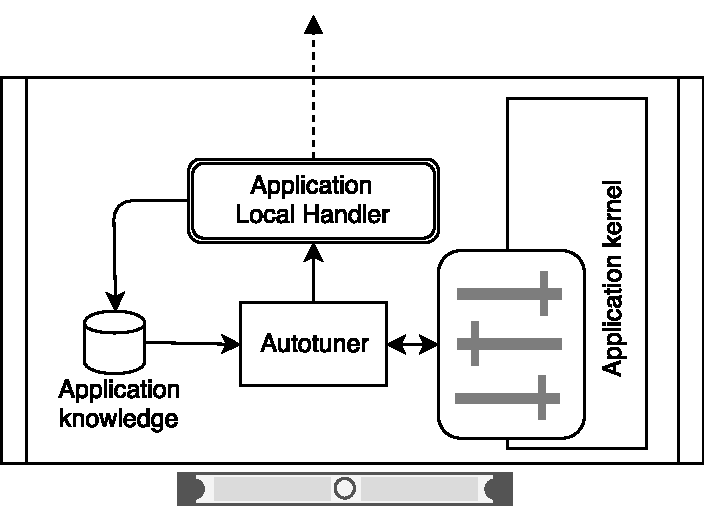
\includegraphics[scale=0.5]{autotuning}
	\caption{The architecture of the local application handler.}
	\label{fig:autotuner}
\end{figure}

The local application handler has three main goals: 1) it provides to the remote application handler information about the actual application, 2) it manages the mARGOt application knowledge to perform a DSE, and 3) provides to mARGOt the final application knowledge.

\prettyref{fig:autotuner} shows the architecture of the local application handler.
While the mARGOt autotuner is synchronous with respect to the execution flow of the target application, the local application handler is a separate thread that communicates with the remote application handler.
In particular, after the initialization, it notifies the existence of a new instance of the application to the server and then it waits for messages.

If the server has no information of this application, the local handler send to the remote handler all the required information.
If the server ask to this client to explore a configuration, the local handler manage the application knowledge to force mARGOt on selecting the given configuration.
If the server send the application knowledge, the local handler replace the old one with the new one.
The only synchronous operation, with respect to the application, happens after each elaboration when mARGOt sends to the remote handler the observed performance of the application.


From the integration point of view, if we are using mARGOt the high-level interface, no additional code is exposed to the end-user.
However, all the required information must be defined in the adaptation configuration file, as described in the mARGOt heel user guide.

\section{How to start the remote application handler}

Since the AGORA application handler implementation requires several dependencies, by default is disabled.
It is possible to enable it, using the cmake flag \textit{-DWITH\_AGORA=ON}.
The build system will automatically download and compile the Cassandra C/C++ client and the Apache Paho MQTT client library.

The remote handler executable is named \textit{agora} and expose several flags to configure its behavior.
Please, use the \textit{--help} command option to have the full list.
In particular, it is possible to configure parameters of the MQTT connection, parameters to the storage connection and the parameters of AGORA itself.

For the MQTT connection, it is possible to specify the url of the broker, the username and password required to authenticate to the broker (if needed) and the communication quality of service.
For the storage conncetion, it is possible to specify the url of one cluster of the databse, and the usename and password required for the authentication (if needed).
You need to start the MQTT broker and the Cassandra database before of running the AGORA application handler.

The server requires only two parameters to successfully start its execution: the workspace folder and the plugin folder.
The workspace folder is the path where the application is able to store files to generate the application knowledge, while the plugin folder is the path to the available plugins.
The standard ones, shipped with AGORA, are located in \textit{<repository\_root>/agora/plugins}.






\end{document}
